
%%% Local Variables:
%%% LaTeX-command: "pdflatex --shell-escape"
%%% End:

\documentclass[11pt]{article}
\usepackage[utf8]{inputenc}
\usepackage[T1]{fontenc}
\usepackage{graphicx}
\usepackage{grffile}
\usepackage{longtable}
\usepackage{wrapfig}
\usepackage{rotating}
\usepackage[normalem]{ulem}
\usepackage{amsmath}
\usepackage{textcomp}
\usepackage{amssymb}
\usepackage{capt-of}
\usepackage{hyperref}
\hypersetup{colorlinks=true, linkcolor=black}
\setlength{\parindent}{0in}
\usepackage[margin=0.8in]{geometry}
\usepackage[spanish]{babel}
\usepackage{mathtools}
\usepackage{palatino}
\usepackage{fancyhdr}
\usepackage{sectsty}
\usepackage{engord}
\usepackage{parskip}
\usepackage{minted}
\usepackage{cite}
\usepackage{graphicx}
\usepackage{setspace}
\usepackage[compact]{titlesec}
\usepackage[center]{caption}
\usepackage{placeins}
\usepackage{color}
\usepackage{amsmath}
\usepackage{bm}
\usepackage{subfigure}
\usepackage{todonotes}
\usepackage{pdfpages}
% \titlespacing*{\subsection}{0pt}{5.5ex}{3.3ex}
% \titlespacing*{\section}{0pt}{5.5ex}{1ex}
\author{Luis Antonio Ortega Andrés\\Antonio Coín Castro}
\date{}
\title{Fingerprint Biometrics Lab - Report\\\medskip
\large APRENDIZAJE PROFUNDO PARA PROCESAMIENTO DE INFORMACIÓN BIOMÉTRICA}
\hypersetup{
 pdfauthor={Luis Antonio Ortega Andrés},
 pdftitle={},
 pdfkeywords={},
 pdfsubject={},
 pdflang={Spanish}}

\begin{document}

\maketitle

\section{Exercise 1}
\textbf{a) } \emph{Copy here the two fingerprint images provided as examples (\texttt{example1\_1} and \texttt{example1\_2})}.

\begin{figure}
  \centering
       \begin{subfigure}[b]{0.2\textwidth}
         \centering
         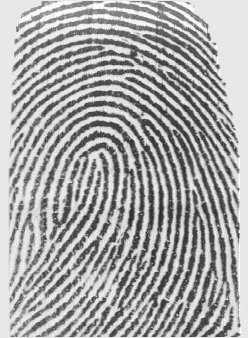
\includegraphics[scale=0.3]{example1_1.png}
         \caption{Example1\_1}
     \end{subfigure}
     \begin{subfigure}[b]{0.2\textwidth}
         \centering
         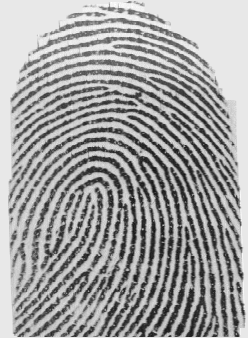
\includegraphics[scale=0.3]{example1_2.png}
         \caption{Example1\_2}
     \end{subfigure}
\end{figure}

\textbf{b) } \emph{How many macro-singularities do you observe in each fingerprint?}

\textbf{c) } \emph{Mark the macro-singularities in the images (deltas and loops).}

\section{Exercise 2}

\textbf{a) }\emph{Execute the provided code for Fingerprint Enhancement and paste the resulting image here:}

\textbf{b) }\emph{What differences do you observe with respect to the original fingerprints?}

\section{Exercise 3}

\textbf{a) }\emph{Execute now the code for Quality Maps, and past the resulting quality maps:}

\textbf{b) }\emph{What is the range of values for these quality maps?}

\textbf{c) }\emph{What kind information (apart from the quality) can be inferred from such code?}

\section{Exercise 4}

\emph{Execute the code in order to show the Binarized Fingerprint and the Segmented Fingerprint. Apply different values of quality threshold (0.1, 0.3, 0.6, 0.9) and paste here the resulting images:}

\section{Exercise 5}

\textbf{a) }\emph{Execute the code for generating the Fingerprint Skeleton and the Minutiae Extractor. Paste the resulting images for the original values window=5 and margin=5.}

\textbf{b) }\emph{Search heuristically by looking at the images for the optimal values of parameters window and margin. Paste the resulting images with your optimal parameters and justify your decision.}

\section{Exercise 6}

\textbf{a) }\emph{Execute the code corresponding to the Minutiae Validation for window=5 and margin=5.  Paste the resulting image including the minutiae extracted (red crosses) and validated (blue circles) of both fingerprints. }

\textbf{b) }\emph{Execute the same code but with the optimal values of parameters window and margin. Paste the resulting image below.}

\textbf{c) }\emph{Do you think it is a good idea to include the Minutiae Validation module? Justify your opinion.}

\section{Extra Exercise}

\emph{In folder \texttt{/ddbb} you have 20 fingerprint images. 19 of them are labeled with the subject identity (e.g., H0001), and 1 is Unknown. Search for the identity of the Unknown fingerprint in the set of 19 labelled reference fingerprints. You can use the provided code \texttt{identification\_1\_19.m} as basis. Paste here the resulting ranked list of scores of the Unknown fingerprint with respect each one of the 19 reference fingerprints.}

\end{document}
